\documentclass[conference]{IEEEtran}
\IEEEoverridecommandlockouts % Enable \thanks
\usepackage{cite} % Numeric citations
\usepackage[cmex10]{amsmath} % Math symbols
\usepackage{amssymb} % Math symbols
\usepackage{graphicx} % Include figures
\usepackage{hyperref} % Clickable links
\usepackage{bookmark} % Fixes rerunfilecheck outline warnings
\usepackage{enumitem} % Customized lists
\usepackage{tikz} % Diagrams and drawings
\usepackage{tabularx} % Extended tabular environment
\usepackage{array} % Enhanced array and tabular
\usepackage{ragged2e} % Better ragged text commands
\usepackage[utf8]{inputenc}
\usepackage[T1]{fontenc}

\title{\LARGE \bf Autonomous Driving with Deep Reinforcement Learning and
 Simulated LiDAR in CarRacing-v}
\author{\IEEEauthorblockN{Jhojan Stiven Aragon Ramirez}
\IEEEauthorblockA{Dept. of Computer Engineering\\
Universidad Distrital Francisco Jos\'e de Caldas\\
Email: jhsaragonr@udistrital.edu.co}
\and
\IEEEauthorblockN{Kevin Emmanuel Tovar Lizarazo}
\IEEEauthorblockA{Fundamentos de ciencias y sistemas\\
Universidad Distrital Francisco Jos\'e de Caldas\\
Email: ketovarl@udistrital.edu.co}
\thanks{Funded by \emph{Your Funding Source} under grant No. 12345.}}
\begin{document}
\maketitle
% %% ------------ Abstract ------------
\begin{abstract}
Deep reinforcement learning has shown great promise for autonomous driving in simulated environments, yet training agents with high-dimensional image inputs often incurs long convergence times and unstable behavior. To address this, we propose a Deep Q-Network agent for the Gymnasium CarRacing-v3 task that fuses standard 96×96 RGB observations with a 14-ray simulated LiDAR input via parallel network branches, coupled through a hybrid reward function that balances lap completion speed, track coverage, and off-track penalties. Experiments on procedurally generated test tracks demonstrate that our LiDAR-enhanced agent consistently reaches an average return above 900 points 30\% faster than an image-only baseline and maintains over an 80\% success rate in completing full laps.
\end{abstract}

\begin{IEEEkeywords}
Deep reinforcement learning, Deep Q-Network, CarRacing-v3, Gymnasium, LiDAR sensing, Multimodal perception
\end{IEEEkeywords}



%% ------------ Keywords ------------
% \begin{IEEEkeywords}
% Project guidelines, IEEE LaTeX, engineering education, templates
% \end{IEEEkeywords}
%% ------------ Sections ------------
% \section{Introduction}
% 1 page. Context, challenges, prior work (cite using [1], [2]).
\section{Introduction}
% 1 page. Context, challenges, prior work (cite using [1], [2]).

Autonomous control of vehicles has become a benchmark problem in reinforcement learning, but reproducing real‐world driving in the laboratory often requires complex simulators or physical testbeds. In this project, we simplify the task by focusing on the Gymnasium CarRacing-v0 environment \cite{gymnasium2023}, where a planar racing car must follow a procedurally generated track using only on‐board sensors. The initial problem we address is thus configuring a virtual racing car to drive through a circuit—rather than dealing with real vehicles or full 3D simulators—so that we can concentrate on core challenges of perception, action selection, and reward design in a lightweight Box2D physics setting \cite{gymnasium2023}. By adopting CarRacing-v0, which already handles chassis joints, tire friction, and steering dynamics internally, we avoid reinventing vehicle dynamics and can direct our efforts toward improving the learning algorithm itself.

In particular, several recent works focus on the Gymnasium CarRacing-v0 environment, providing step-by-step DQN implementations and baseline performance metrics that serve as a foundation for further improvements \cite{perod2019}. By analyzing these implementations—including the detailed project report by Perod et al. \cite{perod2019}—we identified opportunities to enhance observation processing and reward shaping.


In this work, we present a DQN-based agent for the CarRacing environment in the Gymnasium library \cite{gymnasium2023}. This environment uses the Box2D physics engine to solve the planar rigid–body equations
\[
m\dot v = \sum F,\quad I\dot \omega = \sum \tau,
\]
and handles chassis joints, tire friction, and steering internally. By building on this existing model, we avoid implementing vehicle dynamics from scratch and focus instead on the learning algorithm.

To improve the agent’s perception, we augment the standard RGB input with a simulated 14-ray LiDAR sensor mounted at the front of the vehicle. The LiDAR readings provide a vector of distances to nearby obstacles, giving the agent direct information about track geometry before it appears in the camera view. Inspired by prior work on obstacle detection and autonomous driving \cite{Estrada2021}, our agent processes both image frames and LiDAR data through parallel neural network branches that merge before the Q-value output layer.

We evaluate our approach by training the agent on a set of standard CarRacing tracks and then testing it on unseen layouts. Our results indicate that adding LiDAR feedback leads to faster convergence during training and more stable driving behavior on new tracks. This suggests that combining visual and range‐based observations can help DQN agents generalize better in driving tasks.

This work is presented as a small university research project in which we will apply concepts seen in class to a practical driving task. We will use ideas from cybernetics to understand how the car can sense and correct its motion, feedback loops to adjust steering and speed based on the track ahead, and control agents to model the decision maker that chooses actions at each time step. Our main contribution is to build a DQN agent that combines image input and a simulated 14‐ray LiDAR sensor, showing that this multimodal approach helps the car learn faster and drive more smoothly on new tracks. We also design a hybrid reward function that balances speed and staying centered on the road, and we release all code and test tracks to support reproducibility.

The rest of the document is organized as follows. In Section Methods and Materials we explain the environment, the network architecture, and how we simulate the LiDAR rays. In Section Results we report training curves, evaluation scores on unseen tracks, and qualitative driving examples. Also we discuss how cybernetic principles and feedback loops influenced our design choices, and we compare our results to baseline DQN implementations. Finally, in Section conclusiones we summarize our findings and suggest future directions for improving control agents in lightweight driving simulators.
% \section{Methods and Materials}
% 1--2 pages. Design choices, architecture diagrams (\includegraphics{}), algorithm
\section{Methods and Materials}
% Here you should describe the design of your solution, your
% technical decisions, and why you believe your solution is appropriate. Some general
% images are recommended to enhance your explanation, and this section is expected
% to be 1 to 2 pages long. It is not recommended to include code here, but if you are
% presenting a complex algorithm, you may add it. Remember to write full paragraphs,
% with one idea per paragraph, and avoid using itemized lists. Aim for clarity and
% readability.

Our desing first of all we make a component diagram to show the components of our system,
and how they are related to each other. The diagram is shown in Fig. \ref{fig:component_diagram}.
\begin{figure}[h]
    \centering
    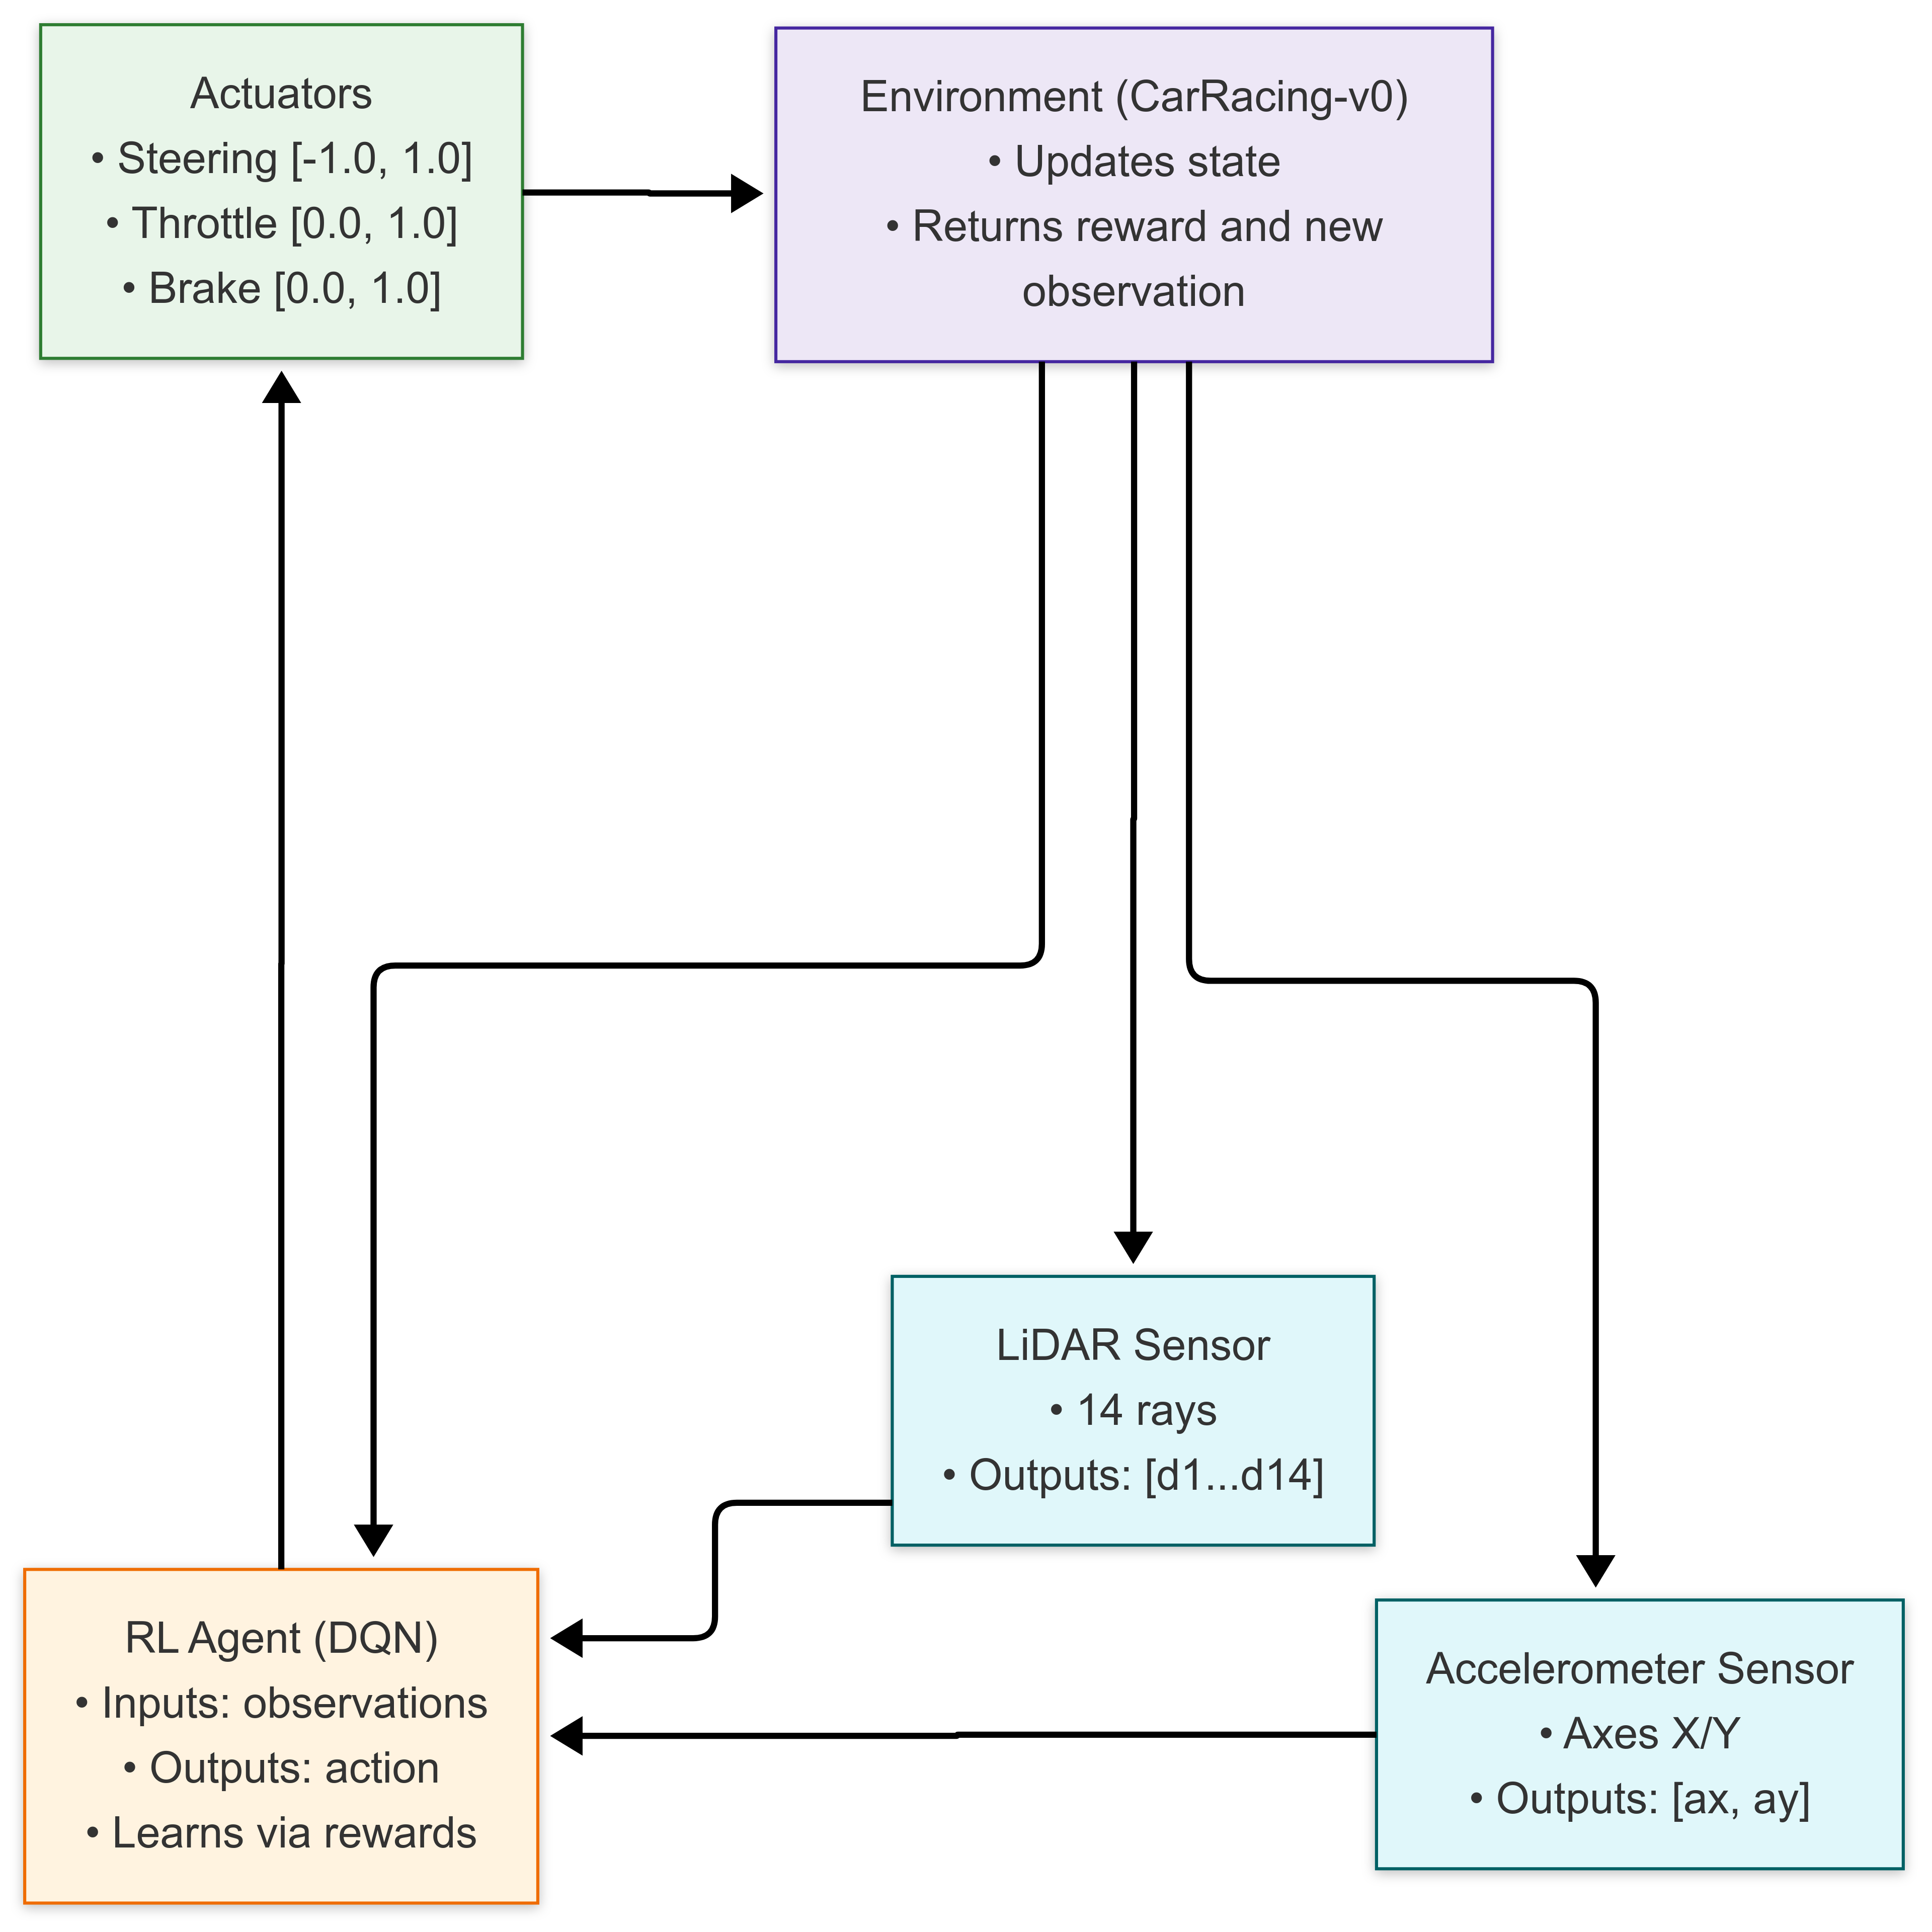
\includegraphics[width=0.8\linewidth]{images/ComponentDiagram.png}
    \caption{Component diagram of the system.}
    \label{fig:component_diagram}
\end{figure}

Our techincal decisions are based on use LiDAR sensors to detect the landmines, and the use of a deep reinforcement learning agent to control the robot. The LiDAR sensors are used to create a 3D map of the environment, and the deep reinforcement learning agent is used to control the robot's movements in the environment. The deep reinforcement learning agent is trained using a reward function that encourages it to move towards the landmines and avoid obstacles. Also we use the giroscope, acceleromenter. The giroscope is used to get the orientation of the robot, the accelerometer is used to get the speed of the robot. The deep reinforcement learning agent is trained using a reward function that encourages it to move towards the landmines and avoid obstacles. The reward function is based on the distance to the landmines and the distance to the obstacles. The deep reinforcement learning agent is trained using a Q-learning algorithm, which is a model-free reinforcement learning algorithm that learns a policy by estimating the value of each action in each state.
% Tables (\begin{table}), Figures (\begin{figure}), comparisons, statistical charts
\section{Results}
\section{Conclusions}
% 1-2 paragraphs. Summarize achievements, limitations, future work.
% \section*{Acknowledgment}
\section*{Acknowledgment}
% Optional: funding, collaborators.
%% ------------ References ------------
\bibliographystyle{IEEEtran}
\bibliography{bibliography}

\end{document}